\documentclass[a4paper, 12pt]{article}
\usepackage{graphicx}
\title{TDT4258 --- Exercise 1}
\author{Per Bachmann, Imre Kerr, Kristian Volden}
\begin{document}
\maketitle
\begin{abstract}
In this exercise, we develop a simple program for an EFM32 Giant Gecko microcontroller. The program lets the user manipulate a row of LEDs using buttons on a game pad. Low energy modes and interrupts are used to reduce power consumption.
\end{abstract}
\section{Introduction} % (fold)
\label{sec:introduction}

% section introduction (end)

\section{Description and Methodology} % (fold)
\label{sec:description_and_methodology}
    \subsection{Description of Program} % (fold)
    \label{sub:description_of_program}
        The functionality of the program is very simple. A single LED will be lit on the gamepad, and the user can press button 1 and 3 (``left'' and ``right'') to move the light left or right.

        A few things must be set up before the main program logic can begin. This is all included in the compendium, but is duplicated here for completeness.

        \begin{enumerate}
            \item Enable GPIO clock in CMU.
            \item Enable interrupts from the GPIO (both even and odd pins).
            \item Set port A pin 8-15 (the LEDs) as output with high drive strength.
            \item Set port C pin 0-7 (the buttons) as input with glitch filter.
            \item Enable pull-up resistors for port C pin 0-7.
            \item Enter sleep mode.
        \end{enumerate}

        Before entering sleep mode, the value \texttt{0xFEFEFEFE} is written to a register and then to port A output. This corresponds to one LED being turned on. From then on, the GPIO interrupt handler will detect if button 1 or 3 has been pressed. If so, it rotates this value one position in the appropriate direction and writes it to output. Since we want to rotate with a period of 8, but the registers are 32 bits, we duplicate the output value four times.

        In the interrupt handler, we must clear the GPIO interrupt flag register by writing \texttt{0xFF} to \texttt{GPIO\_IFC}. We found that this has to happen at the start of the handler, otherwise a second interrupt could be triggered while the handler is running.
    % subsection description_of_program (end)

    \subsection{Methodology} % (fold)
    \label{sub:methodology}
        Our methodology was as follows:
        \begin{enumerate}
            \item Get the hardware and uploading working (Exercise 0).
            \item Write a program that turns on some LEDs.
            \item Modify it to use buttons as well. This version used a busy loop to constantly write the button state to the LEDs.
            \item Modify it to do the same thing, only with interrupts.
            \item Write the final functionality for the program. Having gotten GPIO and interrupts working, this step was easy once we remembered how boolean logic works.
            \item Test the program and fix any problems.
        \end{enumerate}
    % subsection methodology (end)
% section description_and_methodology (end)

\section{Results and Tests} % (fold)
\label{sec:results_and_tests}
	\subsection{Functional Tests} % (fold)
	\label{sub:functional_tests}
		\begin{enumerate}
			\item Pressing the left or right buttons should make the light move left or right, respectively. \\
				  Result: It does.
			\item The buttons should not glitch, i.e. a press should not be registered twice.
				  Result: This did happen occasionally.
		\end{enumerate}
		For the last one, our theory is that the built-in glitch filter in the EFM32GG has a period that is too short (20-50ns according to the data sheet). Since it is implemented in hardware, this period isn't user configurable.
	% subsection functional_tests (end)

	\subsection{Power Consumption} % (fold)
	\label{sub:power_consumption}
		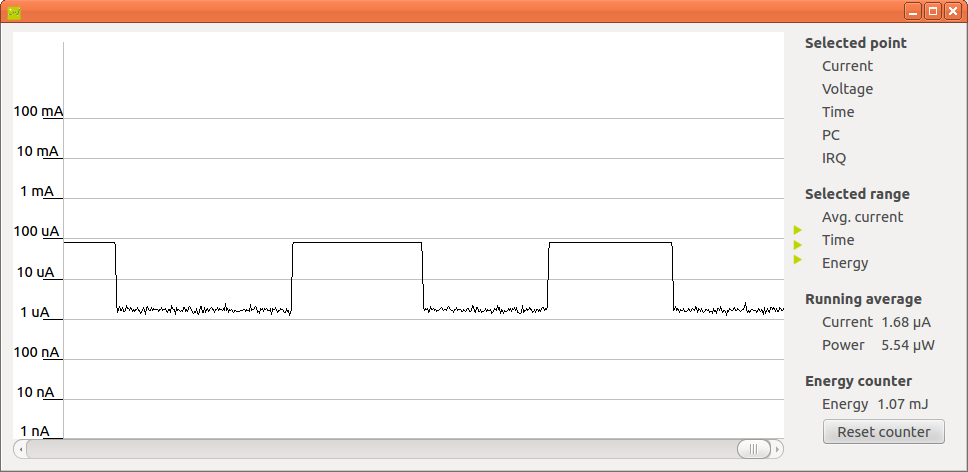
\includegraphics{eaprofiler}
	% subsection power_consumption (end)
% section results_and_tests (end)

\section{Evaluation of Assignment} % (fold)
\label{sec:evaluation_of_assignment}

% section evaluation_of_assignment (end)

\section{Conclusion} % (fold)
\label{sec:conclusion}

% section conclusion (end)

\section{References} % (fold)
\label{sec:references}

% section references (end)
\end{document}